\documentclass{article}

% Packages for code listing and syntax highlighting
\usepackage{amsmath}
\usepackage{amssymb}
\usepackage{bm}
\usepackage{listings}
\usepackage{xcolor}
\usepackage[margin=3cm]{geometry} % Adjust the margin value as desired
\usepackage{setspace}
\usepackage{tikz}
\usepackage{graphicx}
\usepackage{float}
\usepackage{textcomp}
\usepackage{multicol}
\usepackage{enumitem}
\usepackage{circuitikz}
\usepackage{url}
\usepackage{amsthm}
\usepackage{tcolorbox}

\onehalfspacing

% Define the color theme
\definecolor{codebackground}{RGB}{242, 242, 242}
\definecolor{codekeyword}{RGB}{0, 0, 255}
\definecolor{codecomment}{RGB}{63, 127, 95}
\definecolor{codestring}{RGB}{163, 21, 21}

% Code listing style for all languages
\lstdefinestyle{mystyle}{
    backgroundcolor=\color{codebackground},
    basicstyle=\footnotesize\ttfamily,
    keywordstyle=\color{codekeyword}\bfseries,
    commentstyle=\color{codecomment}\itshape,
    stringstyle=\color{codestring},
    numbers=left,
    numberstyle=\tiny\color{codecomment},
    stepnumber=1,
    numbersep=8pt,
    showstringspaces=false,
    breaklines=true,
    frame=single,
    frameround=none,
    framesep=5pt,
    rulecolor=\color{codebackground},
    tabsize=4,
    captionpos=b,
    xleftmargin=15pt,
    xrightmargin=15pt
}

% Set the default style for code listings
\lstset{style=mystyle}

\newtheoremstyle{problemstyle}
  {0.5em} % Space above
  {0.5em} % Space below
  {} % Body font
  {} % Indent amount
  {\bfseries} % Theorem head font
  {} % Punctuation after theorem head
  {.5em} % Space after theorem head
  {} % Theorem head spec (can be left empty, meaning 'normal')

\theoremstyle{problemstyle}
\newtheorem{problem}{Problem}

\newenvironment{boxedproblem}[1]
{\begin{tcolorbox}[colback=white, colframe=black, boxrule=0.5pt]\noindent\textbf{Problem #1.}}
{\end{tcolorbox}}

% Define your document content
\begin{document}

\title{Problem Set X}
\author{Abyan Majid}
\date{\today}
\maketitle

% --------------------------------------------------------------------

\begin{boxedproblem}{1}
State the problem here.
\end{boxedproblem}

\textbf{Solution:}
\begin{itemize}[label={},leftmargin=1.25cm,nosep]
    \item First step
    \item Second step
    \item Third step
\end{itemize}

% --------------------------------------------------------------------

\begin{boxedproblem}{2}
State the problem here.
\end{boxedproblem}

\textbf{Solution:}
\begin{itemize}[label={},leftmargin=1.25cm,nosep]
    \item First step
    \item Second step
    \item Third step
\end{itemize}

% --------------------------------------------------------------------

\begin{boxedproblem}{3}
State the problem here.
\end{boxedproblem}

\textbf{Solution:}
\begin{itemize}[label={},leftmargin=1.25cm,nosep]
    \item First step
    \item Second step
    \item Third step
\end{itemize}

% --------------------------------------------------------------------

\section{Code Example}

\begin{lstlisting}[language=Python, caption={Example Code Block}]
def hello_world():
    print("Hello, world!")
\end{lstlisting}

\section{Image Example}

\begin{figure}[H]
    \centering
    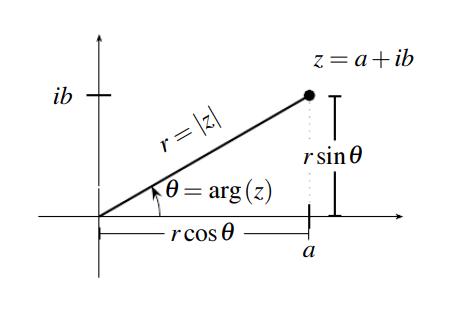
\includegraphics{../!assets/MATH1021-003-fig1.png}
    \caption{Polar form of complex numbers}
\end{figure}

\end{document}